%************************************************
\chapter{Results}\label{ch:Results}
%************************************************

In this section we will explore the experimental results of this work. First we
will focus on the startup time of containers, and we will make two different
comparison for this metric. First we will compare the use of CVMFS structured
as explained in this work as content distribution mechanism against the
standard way of distributing content. Then we will compare a more naive use of
CVMFS without the use of \textit{super-directories} and sub-catalogs against
the proposed file system structure that instead exploit the sub-catalog
mechanism. 

Then we will compare the use of bandwidth, again we will make two different
comparison. The first will compare the use of CVMFS as content distribution
layer against the normal distribution mechanism used for containers base on
Docker registries. Then we will compare the use of the proposed file system
structure against a file system, still hosted in CVMFS, but without the use of
sub-catalogs. 

Finally we will measure the complexity of managing the proposed file system
structure.

\section{Containers startup time}

In the first part of this section we explore the startup time of container
hosted in CVMFS using the proposed structure against containers hosted in a
normal file system. The second part of this section will analyze the startup
time of container hosted in CVMFS using the proposed file system structure
against hosting containers in CVMFS but without the use of
\textit{super-directories} and subcatalogs.

On both parts we will use a representative use case, we will start the standard
python container, start the python interpreter and immediately quit the
interpreter itself executing the \textit{quit()} command. We decide to use this
use case since it requires to have access to the python interpreter in the
container, which is an executable of not negligible size: 3.4MB. Moreover, we 
chose the standard python image because is a widely known image used during both
development and production work. The size of the whole image is of roughly 923MB.

All the measurements are collected using the standard unix util \textit{time}.

\subsection{Use of CVMFS vs. Standard containers distribution mechanism}

For this analysis we propose 8 scenarios that we synthesize in Table
\ref{tab:benchmark} and on the graph of Figure \ref{fig:startup-time}. The
\textit{Thin-Image on CVMFS} row represent the startup time of containers which
content is hosted in the CVMFS architecture discussed in this work. The
\textit{Default} columns represent the start up time of containers using the
default distribution system based on Docker Registries.

\begin{table}[]
\begin{tabular}{|l|l|l|l|l|l|}
\hline
\multicolumn{2}{|l|}{\multirow{2}{*}{}}            & \multicolumn{2}{l|}{Cache} & \multicolumn{2}{l|}{No Cache} \\ \cline{3-6} 
\multicolumn{2}{|l|}{}                             & Avg          & STD         & Avg            & STD          \\ \hline \hline
\multirow{2}{*}{Thin-Image on CVMFS} & Singularity & 10.31        & 4.38        & 29.13          & 4.02         \\ \cline{2-6} 
                                     & Docker      & 96.74        & 5.40        & 180.02         & 35.13        \\ \hline \hline
\multirow{2}{*}{Default}               & Singularity & 7.38         & 2.07        & 1884.76        & 366.84       \\ \cline{2-6} 
                                     & Docker      & 95.26        & 5.29        & 1279.21        & 168.99       \\ \hline
\end{tabular}
\caption{Benchmark of startup time of a containers, the first number is the average while the second is the standard deviation. The units are in hundredths of seconds. $n = 100$}
\label{tab:benchmark}
\end{table}

\begin{figure}[]{}
    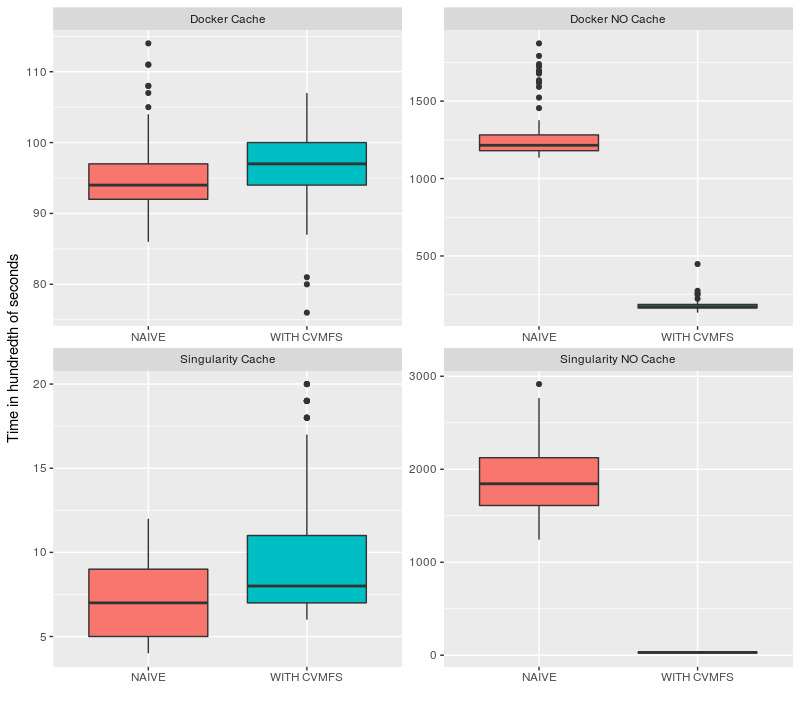
\includegraphics[width=\textwidth]{gfx/plot-startup-time}
        \caption{Startup times of the containers served using the proposed architecture and served using the standard Docker Registries.}
        \label{fig:startup-time}
\end{figure}


We can see that the use of CVMFS is a huge help when the cache is not
available, moreover its overhead is almost negligible when the cache is
present. Is interesting to know that the containers hosted in CVMFS without
cache starts in an amount of time whose order of magnitude is comparable to the
containers hosted naively but using cache (4 times slower in the case of
Singularity and 2 times slower in the case of Docker.)

\subsection{Use of the proposed file system structure vs. using CVMFS without sub catalogs}

In this section we are going to analyze how the use of sub-catalogs affect the
startup performance. Differently from the above test, in this case the
differences lies mostly on the uncached case. Indeed when the sub-catalog is
already downloaded and cached in the local client the time difference is
negligible. For this test, as base case we use the containers served using the file
system structure presented in this work, on the other side we serve the
containers without using sub-catalogs. Moreover, in the case without
sub-catalogs we present the case where the whole repository contains 10,
20, 30 and 40 images.

We used the Singularity runtime for this test that being faster to start up is less
influenced by the run time overhead. Moreover, the base case is equivalent to
the case showed in the previous test, using the Singularity run time, served by
CVMFS without cache. Hence the base case we are comparing is the one with
average startup time of 29.12 hundredths of second and standard deviation of
4.02 hundredths of seconds. 


% Please add the following required packages to your document preamble:
% \usepackage{multirow}
\begin{table}[]
\begin{tabular}{|l|ll|ll|ll|ll|}
\hline
Images in Catalogs            & \multicolumn{2}{l|}{10}   & \multicolumn{2}{l|}{20}    & \multicolumn{2}{l|}{30}    & \multicolumn{2}{l|}{40}    \\ \hline
Size of subcatalog            & \multicolumn{2}{l|}{67MB} & \multicolumn{2}{l|}{127MB} & \multicolumn{2}{l|}{188MB} & \multicolumn{2}{l|}{249MB} \\ \hline
\multirow{2}{*}{Startup time} & AVG          & STD        & AVG           & STD        & AVG           & STD        & AVG           & STD        \\ \cline{2-9} 
                              & 57.61        & 6.01       & 88.76         & 7.52       & 129.50        & 15.95      & 150.42        & 29.84      \\ \hline
\end{tabular}
\caption{Startup time of Singularity containers with the respect of the subcatalog size. The units are in hundredths of seconds. $n = 100$}
\label{tab:benchmark-catalog}
\end{table}

\begin{figure}[]{}
    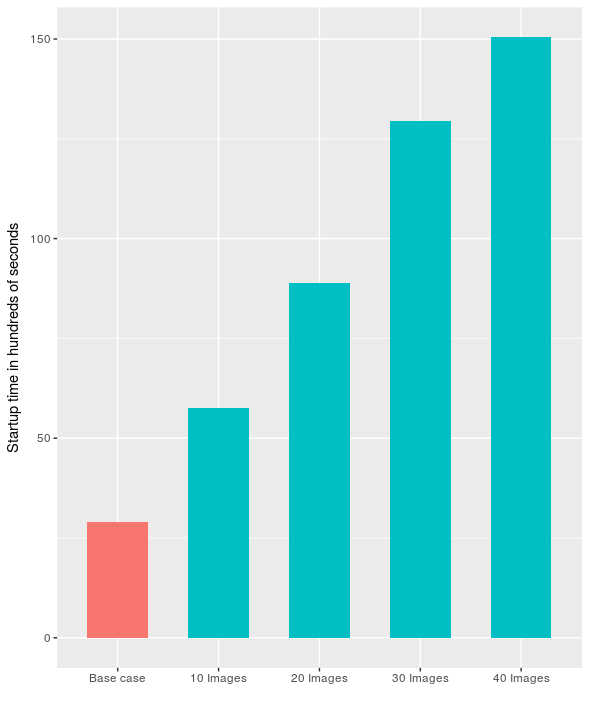
\includegraphics[width=\textwidth]{gfx/runtime-catalog}
        \caption{Comparison of the containers startup times with the proposed file system structure and without the use of subcatalogs.}
        \label{fig:startup-time}
\end{figure}


On Table \ref{tab:benchmark-catalog} we can see how, on increasing the images
in the catalogs, hence in increasing the size of the subcatalog the
time to start a containers without using the cache increases as well.

Indeed, the catalog need to be downloaded completely before that it can be
used, hence increasing the catalog size impact directly with the startup time
of the containers. Which is the reason why we decide to use the concept of
\textit{super directories}.

\section{Containers bandwidth use}

In this section we are going to show how the presence of sub-catalogs affect the bandwidth usage. Also in this case we run the python image calling immediately the \textit{quit()} command.

Similarly to the above case we present the case where the catalogs contains 10, 20, 30 and 40 images and we compare it with the baseline case, hence with the case that use the structured showed in this work.

The results are show on Table \ref{tab:bandwith-catalog} and on Figure \ref{fig:bandwidth-usage}

\begin{figure}[]{}
    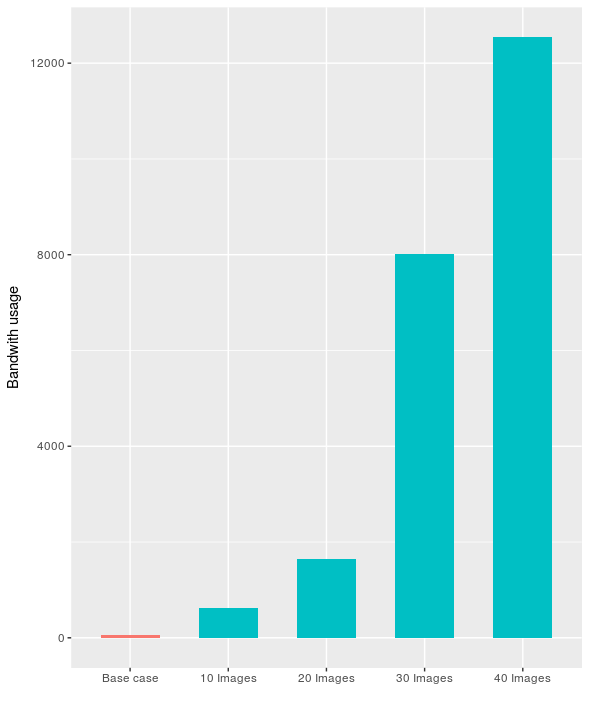
\includegraphics[width=\textwidth]{gfx/bandwidth-catalog}
        \caption{Comparison of the bandwidth with the proposed file system structure and without the use of subcatalogs.  }
        \label{fig:bandwidth-usage}
\end{figure}


\begin{table}[]
\begin{tabular}{|l|l|l|l|l|l|}
\hline
                & Base Case & 10  & 20   & 30   & 40    \\ \hline
Bandwidth Usage & 64.25     & 624 & 1651 & 8020 & 12540 \\ \hline
\end{tabular}
\caption{Comparison of the bandwidth used to start the containers 100 times with and without use of subcatalogs. Units in MB.}
\label{tab:bandwith-catalog}
\end{table}

Also in this case we can see how structuring the file system using sub-catalogs
improves the bandwidth efficiency.

\section{Space Requirement}

By default CVMFS stores all its content in \texttt{/srv}, hence the most
reliable way to obtain the size of the repository is to analyze the storage
used under \texttt{/srv}. The storage required for the whole repository is of
~14G calculate with the \texttt{du} unix utility.

We than obtain the size of the two hidden folder \textit{.layers} and
\textit{.flat} using the `cvmfs\_server list-catalogs` command which provides us
with the number of files in each catalog and the number of bytes that each
catalog manage. We finally show all the measurement on Figure \ref{tab:size-of-repo}.

\begin{table}[]
\begin{center}
\begin{tabular}{|l|lll|}
\hline
        & Storage & .flat & .layers \\ \hline
        Size & 14 & 24    & 26      \\ \hline
\end{tabular}
\end{center}
\caption{Apparent size in GB of the two folder \textit{.layers} and \textit{.flat}}
\label{tab:size-of-repo}
\end{table}

We can see that the Content-Addressable-Storage used by CVMFS helps a lot by
reducing the amount of space required to host the repository by half, which
make sense since the \textit{.layers} and the \textit{.flat} contains the exact
same files.

\section{Complexity}

In order to estimate the complexity of managing the file-system we decided to
use the cyclomatic complexity of the tool that create and manage the
file-system itself that we discuss on Chapter \ref{ch:Implementation}. We used
\textit{gocylo} \cite{gocyclo} a command line tool that calculates the
cyclomatic complexity of functions written in the Go(lang) language. We show
the result of the cyclomatic analysis on Table \ref{tbl:cyclomatic}.

\begin{table}[]
\begin{tabular}{|l|l|}
\hline
\multicolumn{1}{|r|}{Cyclomatic Complexity} & \multicolumn{1}{r|}{Function} \\ \hline
37 & ConvertWish \\ \hline
15 & ParseImage \\ \hline
14 & AddManifestToRemoveScheduler \\ \hline
12 & GarbageCollectSingleLayer \\ \hline
12 & (Image).GetChanges \\ \hline
12 & (Image).downloadLayer \\ \hline
11 & SaveLayersBacklink \\ \hline
11 & IngestIntoCVMFS \\ \hline
9 & requestAuthToken \\ \hline
9 & CreateSymlinkIntoCVMFS \\ \hline
9 & RemoveDirectory \\ \hline
8 & (Image).GetLayers \\ \hline
7 & FindImageToGarbageCollect \\ \hline
7 & (Image).GetReference \\ \hline
6 & AlreadyConverted \\ \hline
6 & getBacklinkFromLayer \\ \hline
6 & (*execCmd).Start \\ \hline
\end{tabular}
\caption{Result of the cyclomatic complexity analysis, only function with complexity greater or equal to 3 are shown}
\label{tbl:cyclomatic}
\end{table}

While the cyclomatic complexity is very high it is important to note that
idiomatic golang codes requires to manually check every possible error returned
by other functions, all these checks increase dramatically the cyclomatic
complexity of the code. Indeed there are 19 error check without any logic in
the code but simply returning early in the ConvertWish function.


